% Tabels of nodes and triangled visited. Perhaps some statistics over
% wasted iterations by threads waiting for other threads in the warp
% to finish. The high triangle count pr leaf optimization may be
% related to this and makes using highly optimized splitting plane
% calculations in the lower nodes useless.

\chapter{Results}\label{chp:results}

\chapterquote{It’s hardware that makes a machine fast. It’s software
  that makes a fast machine slow.}{Craig Bruce}

% Intro

In this chapter I will compare the speed and quality of different kd-tree
construction schemes implemented as part of this thesis.

% Hardware

The implementations have been tested on a dual core Intel Core i7 2.66GHz CPU
with 4GB RAM. The GPU used is an NVIDIA 330M with CUDA Compute Capability 1.2, 6
multiprocessors running at 1.1GHz and 512MB RAM. CUDA 3.1 was installed on the
machine. All tests where performed with a screen resolution of 640x480, which
equals 307200 primary rays traced into the scene.

\begin{figure}
  \centering
  \subfloat[The Cornell Box - 36 Triangles.]{
    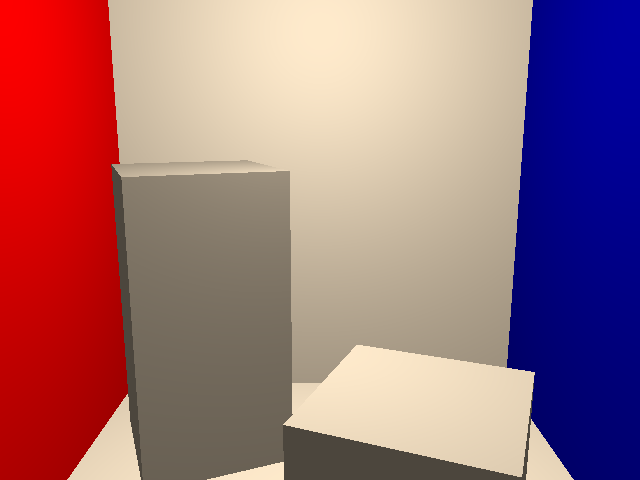
\includegraphics[width=0.3\textwidth]{cornellBox}
  }
  \subfloat[The Reflecting Stanford Dragon - 203k Triangles.]{
    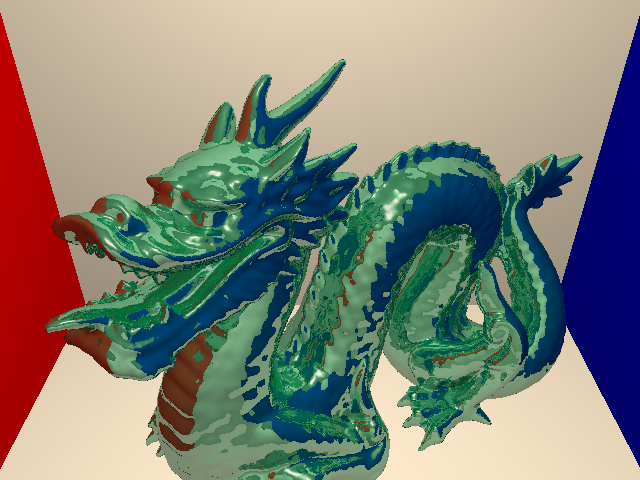
\includegraphics[width=0.3\textwidth]{semiReflectingDragon}
  }
  \subfloat[Sponza - 279k Triangles.]{
    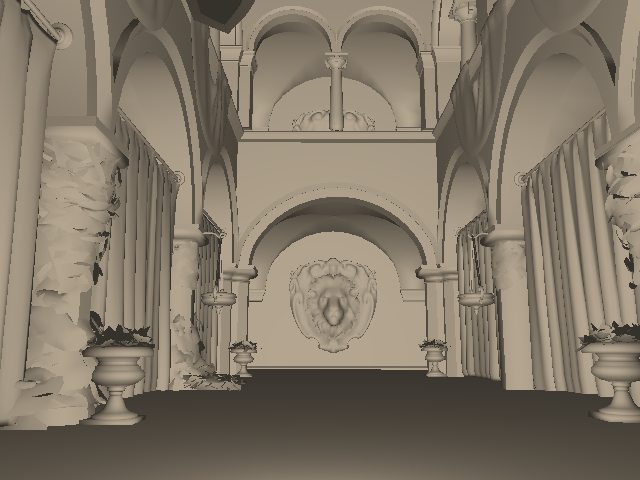
\includegraphics[width=0.3\textwidth]{sponza}
  }
  \caption[Test scenes.]{The 3 test scenes used in this chapter.}
  \label{fig:testScenes}
\end{figure}

% Test scenes: Cornell, reflecting dragon2 and sponza

The tests will be conducted on three different test scenes shown in
\reffig{fig:testScenes}. \textit{The Cornell Box} scene was chosen for its
simplicity. With only 36 triangles the scene should be very fast to render and
allows me to compare the performance of the ray tracer implementations on a
simple scene. The \textit{Sponza} scene was chosen for its complexity. At 279k
triangles it will test both the quality and the construction speed of the
kd-tree constructors in large scenes. The last scene tested is \textit{The
  Reflecting Stanford Dragon} consisting of 203k triangles. The reflecting
geometry in the scene spawns 189572 reflection rays and is used to test
the importance of a high quality kd-tree when more rays than just the primary
are traced.

% Rest of this chapter

In \refsection{sec:evaluateRayTracer} I will evaluate the different ray tracer
implementations and the impact of the optimizations described in
\refsection{sec:hierarchicalTraversal}. I have chosen to implement the
short-stack optimization as a seperat ray tracer, instead of applying it to the
kd-restart ray tracer. This is merely a design decision and has no impact on the
actual results presented below. The overall fastest ray tracer will be used in
the following sections to evaluate the quality of the kd-trees constructed. In
\refsection{sec:evaluateUpperTree} I will compare quality and construction speed
of the different construction schemes for the upper part of the kd-tree. The
upper tree configuration that performs best, will be used in
\refsection{sec:evaluateUpperTree}, where the kd-tree's lower parts will be
constructed using SAH, SSAH and no construction scheme.

As explained in the introduction, the worst-case scenario for a dynamic scene is
a complete reconstruction of the acceleration structure. To ensure that my
implementations are tested against the worst-case scenario, the acceleration
structures are completely rebuild for each image rendered. The best kd-tree
configuration is therefore the one that minimizes the total time spent
constructing the kd-tree and afterwards ray tracing it.


\section{Evaluate Ray Tracers}\label{sec:evaluateRayTracer}

\Reffig{fig:rayTracerEvaluation} shows the time it took the different ray tracer
configurations to render each of the three test scenes. The kd-tree
configuration used to produce kd-trees for the hierarchical ray tracers is
described in the figure's caption.

\newcommand{\tabelMoeller}{
  \begin{tabular}{c}
    Moeller- \\ Trumbore
  \end{tabular}
}

\begin{figure}
  \centering
  \begin{minipage}{\textwidth}
    \centering
    \SetTabelTextSize
    \begin{tabular} {r | c | c | c || c || c || c ||}
      \tabelParam{c}{\textit{Ray} \\ \textit{Tracer:}} &
      \tabelParam{c}{\textit{Ray/triangle}\\\textit{intersection:}} &
      \tabelParam{c}{\textit{Packets:}} &
      \tabelParam{c||}{\textit{Leaf} \\ \textit{skipping:}} &
      \tabelScene{Cornell \\ Box \\ 1.0ms (3)} & 
      \tabelScene{Reflecting \\ Dragon \\ 150ms (49909)} & 
      \tabelScene{Sponza \\ 263ms (98779)}\\
      \hline\hline
      \multirow{4}{*}{Exhaustive\footnote{The exhaustive ray tracer only ray traces the first 4096 triangles in a scene. Even with this hard upper limit it is clear that an exhaustive approach will not work for detailed scenes.}} & 
        \multirow{2}{*}{\tabelMoeller} & No & N/A & 11.2ms & \worstResult{1118ms} & \worstResult{964ms} \\
      \cline{3-7}
      & & 4x8 & N/A & \worstResult{11.6ms} & 1114ms & \worstResult{964ms} \\
      \cline{2-7}
      & \multirow{2}{*}{Woop} & No & N/A & \bestResult{9.3ms} & \bestResult{898ms} & \bestResult{650ms}\\
      \cline{3-7}
      & & 4x8 & N/A & 9.7ms & 903ms & 651ms\\
      \hline
      \hline

      % KD-Restart
      \multirow{8}{*}{KD-Restart} & \multirow{4}{*}{\tabelMoeller} & \multirow{2}{*}{No} & No & 17.9ms & \worstResult{790ms} & \worstResult{592ms} \\
      \cline{4-7}
      & & & Yes & \worstResult{18.1ms} & 486ms & 287ms \\
      \cline{3-7}
      & & \multirow{2}{*}{4x8} & No & 17.2ms & 579ms & 424ms \\
      \cline{4-7}
      & & & Yes & 17.4ms & \bestResult{355ms} & \bestResult{196ms} \\
      \cline{2-7}
      & \multirow{4}{*}{Woop} & \multirow{2}{*}{No} & No & 15.5ms & 690ms & 549ms \\
      \cline{4-7}
      & & & Yes & 15.8ms & 500ms & 287ms \\
      \cline{3-7}
      & & \multirow{2}{*}{4x8} & No & \bestResult{14.6ms} & 495ms & 342ms \\
      \cline{4-7}
      & & & Yes & 14.8ms & \bestResult{355ms} & \bestResult{198ms} \\
      \hline
      \hline
      
      % Short-Stack
      \multirow{8}{*}{Short-Stack} & \multirow{4}{*}{\tabelMoeller} & \multirow{2}{*}{No} & No & 20.0ms & \worstResult{808ms} & \worstResult{595ms} \\
      \cline{4-7}
      & & & Yes & \worstResult{20.2ms} & 503ms & 266ms \\
      \cline{3-7}
      & & \multirow{2}{*}{4x8} & No & 19.5ms & 590ms & 421ms \\
      \cline{4-7}
      & & & Yes & 19.8ms & \bestResult{360ms} & \bestResult{167ms} \\
      \cline{2-7}
      & \multirow{4}{*}{Woop} & \multirow{2}{*}{No} & No & 18.5ms & 738ms & 560ms \\
      \cline{4-7}
      & & & Yes & 18.7ms & 522ms & 270ms \\
      \cline{3-7}
      & & \multirow{2}{*}{4x8} & No & \bestResult{17.8ms} & 523ms & 348ms \\
      \cline{4-7}
      & & & Yes & 18.1ms & 368ms & 171ms \\
      \hline
    \end{tabular}\par
    \vspace{-0.75\skip\footins}
    \renewcommand{\footnoterule}{}
  \end{minipage}
  \caption[Ray tracing results.]{The table shows the time it took different ray
    tracer configurations to render each of the three test scenes.  The bold
    faced render times performed the best for a given ray tracer and scene. The
    ones in red performed the worst. The kd-trees for the scenes were
    constructed with Empty Space Maximization enabled and a threshold of 25\%,
    the triangle/node association scheme employed was Dividing. The threshold
    for the lower tree was 32, but no lower tree was constructed. The number of
    nodes in the kd-tree is reported in parenthesis below the name of the
    scene. The size of the short stack was 4 elements, which has been found to
    perform well in practice.}
  \label{fig:rayTracerEvaluation}
\end{figure}

% Evaluate the ray tracers for the individual scenes

From \reffig{fig:rayTracerEvaluation} it can be seen that the exhaustive ray
tracer generelly performs worst of all the ray tracers. This was to be expected,
since the exhaustive ray tracers time complexity is $O(nm)$ and the hierarchical
ray tracers' are $O(n \log m)$, for $n$ rays and $m$ triangles. As expected
Woop's simpler Triangle/Ray intersection performs better than Moeller-Trumbore's
for all exhaustive ray tracer configurations. The screen space packet
optimization has also been applied to the exhaustive ray tracer, but generelly
causes a small overhead instead of a performance improvement. This was to be
expected, since all rays intersect the triangles in the same order, and
therefore it does not matter which rays are traced together. In the Reflecting
Dragon scene we see a small speed increase when using packets. This may be the
result of fewer warps tracing reflection rays, but can also be caused by an
acceptable deviation in timing precision.

In the Cornell Box scene, the kd-restart implementation performed worse than the
exhaustive ray tracer, even without taking the kd-tree construction time of 1ms
into account. This is not entirely unexpected, since the exhaustive ray tracer
only needs to intersect every ray with 36 triangles, where the kd-restart
implementation needs to first traverse the root node, before it can begin
ray/triangle intersection in leafs that can reference up to 32 triangles. In the
more complex scenes, kd-restart outperformed exhaustive ray tracing by a wide
margin. Unsurprisingly the configuration consisting of Moeller-Trumbore
intersection, no packets and no leaf skipping performed the worst. It was a bit
more surprising to see that with packets and leaf skipping enabled, it did not
matter much if Moeller-Trumbore's or Woop's intersection method was
used. Especially since Woop's intersection test generelly outperformed
Moeller-Trumbore. However, this makes sense since the rays in the same warp are
spatially close and are therefore able to skip most of the leaf nodes they
visit, and thus a lot of intersection computations, before reaching their
intersection point.

The packet size 4x8 was found to perform best and is therefore the only packet
size represented in \reffig{fig:rayTracerEvaluation} to keep the table
simple. In generel enabling Packets decreased rendering time by 27-37\%.

Enabling Leaf Skipping decrased rendering time by 28-54\%. The largest decrease
in rendering time was seen in configurations that used Moeller-Trumbore's
ray/triangle intersection tests, again confirming that Moeller-Trumbore is the
slowest ray/triangle intersectiong compared to Woop's.

The short-stack implementation performed very similar to kd-restart. In the
simple Cornell Box scene it performed slightly worse, due to the overhead of
maintaining a stack. In the Reflecting Dragon scene, it performed roughly
similar to kd-restart and in the Sponza scene it outperformed both the
exhaustive ray tracer, kd-restart and was about 70\% faster than an unoptimized
kd-restart implementation.

Overall the short-stack implementation with Moeller-Trumber intersection,
packets and leaf skipping enabled performed the best. While it may have been
outperformed in the Cornell Box, it was by far the best ray tracer in the
complex Sponza scene. I will therefore use it to evaluate the quality of
kd-trees in the following sections.


\section{Evaluate Upper Tree Creation}\label{sec:evaluateUpperTree}

Since the Cornell Box scene contains so few triangles and only shows that the
exhaustive ray tracer is fastest for extremely simple scenes, I will not be
using it to evaluate the kd-tree constructor configurations. Instead I will only
use the Reflecting Dragon and Sponza scenes.

The results from creating the upper parts of the kd-tree with different
configurations can be seen in \reffig{fig:upperResults}. The entries in the
table shows kd-tree construction time, the time used to render the scene and the
number in parenthesis is the amount of nodes in the constructed kd-tree.


\begin{figure}
  \centering
  \SetTabelTextSize
  \begin{tabular} {c | c | c || c || c ||}
    % Titel bar: Association scheme | empty space maximization | threshold | dragon | sponza
    \multicolumn{1}{c}{\begin{tabular}{c}\textit{Association} \\ \textit{scheme:}\end{tabular}} &
    \multicolumn{1}{c}{\begin{tabular}{c}\textit{Empty Space} \\ \textit{Maximization:}\end{tabular}} &
    \begin{tabular}{c}\textit{Empty}\\\textit{Space} \\ \textit{Threshold:}\end{tabular} &
    \tabelScene{Reflecting \\ Dragon} &
    \tabelScene{Sponza}\\
    \hline\hline % Titel end
    \multirow{4}{*}{Dividing} & No & N/A & \worstResult{146/385ms (38k)} & \worstResult{258/220ms (87k)}\\
    \cline{2-5}
    & \multirow{3}{*}{Yes} & 15\% & 150/376ms (56k) & 263/167ms (104k) \\
    \cline{3-5}
    & & 25\% & \bestResult{150/355ms} (50k) & \bestResult{263/167ms (99k)}\\
    \cline{3-5}
    & & 35\% & 150/357ms (45k) & \bestResult{263/167ms (95k)}\\
    \hline\hline
    \multirow{4}{*}{Box Inclusion} & No & N/A & \worstResult{116/397ms (41k)} & \worstResult{213/241ms (112k)} \\
    \cline{2-5}
    & \multirow{3}{*}{Yes} & 15\% & 121/386ms (59k) & 219/182ms (130k) \\
    \cline{3-5}
    & & 25\% & 121/373ms (53k) & 219/182ms (125k)\\
    \cline{3-5}
    & & 35\% & \bestResult{121/366ms (48k)} & \bestResult{219/180ms (120k)}\\
    \hline
  \end{tabular}
  \caption[Upper tree creation results.]{The entries in the table show the time
    it took to create the kd-tree in milliseconds, the time it took to render
    the scene and the number of nodes in the kd-tree is the number in
    parenthesis. The scene was ray traced using the short stack configuration
    that performed best above. To keep the lower tree construction phase from
    having as little influence on the results as possible, no lower tree will be
    constructed and lower tree threshold has been set to 32. As in
    \reffig{fig:rayTracerEvaluation} the boldfaced text denotes the fastest
    configuration and red the slowest.}
  \label{fig:upperResults}
\end{figure}

From the results it is clear that using the Dividing triangle/node association
scheme produces trees of trees of highest quality. In the Reflecting Dragon
scene, trees build with Dividing are generelly ray traced 10ms, or 2.5\%, faster
and contain 3k fewer nodes than their Box Inclusion counterparts. In the Sponza
scene the difference is even more noticeable at up to 8.7\%. Unfortunatly
producing kd-trees using the Dividing scheme is a lot slower than using Box
Inclusion. In the above scenes this means that while Dividing produces the
highest quality trees, Box Inclusion makes up for its slower ray tracing results
by producing trees up to 19\% faster.

As can be seen on the table, enabling Empty Space Maximization adds 4-6ms to the
kd-tree construction time and a few thousand extra nodes to the tree. Enabling
it also increase the tree quality though and ray tracing improvements lie in the
range of 8\% for the Reflecting Dragon and 24\% in Sponza's great hall. The
substantial increase in Sponza is a direct consequence of all the empty space in
the middle of the scene that the rays have to traverse. As for setting the Empty
Space Threshold, 35\% seems to be marginally better than 25\%. They achieve
roughly the same tree quality, but with a 35\% Empty Space Threshold the tree
becomes 4-10\% smaller than a tree with a 25\% threshold. The tree will thus
take up less memory, which can become important on GPU's where memory is
limited.

Overall configuring the tree constructor to use Box Inclusion and Empty Space
Maximization with a 35\% threshold yielded the best tradeoff between
construction speed and ray tracing time.

\section{Evaluate Lower Tree Creation}\label{sec:evaluateLowerTree}

% Lower node creation

\begin{figure}
  \centering
  \SetTabelTextSize
  \begin{tabular}{c |c | c || c || c ||}
    \tabelParam{c}{\textit{Bit Mask:}} &
    \tabelParam{c}{\textit{Splitting} \\ \textit{Scheme:}} &
    \tabelParam{c||}{$C_N/C_i:$} &
    \tabelScene{Reflecting \\ Dragon} &
    \tabelScene{Sponza}\\
    \hline\hline % Titel end
    \multirow{7}{*}{32bit} & None & N/A & \bestResult{121/357ms (48.1k)} & \bestResult{219/179ms (120k)}\\
    \cline{2-5}
    & \multirow{3}{*}{SAH} & 24 & 273/358ms (48.2k) & 616/180ms (121k)\\
    \cline{3-5}
    & & 16 & 273/359ms (48.3k) & 648/180ms (129k)\\
    \cline{3-5}
    & & 8 & \worstResult{280/358ms (50k)} & \worstResult{775/181ms (167k)}\\
    \cline{2-5}
    & \multirow{3}{*}{SSAH} & 24 & 159/382ms (126k) & 305/201ms (287k)\\
    \cline{3-5}
    & & 16 & 162/393ms (143k) & 309/207ms (313k)\\
    \cline{3-5}
    & & 8 & 165/401ms (168k) & 318/227ms (394k)\\
    \hline \hline
    \multirow{7}{*}{64bit} & None & N/A & \bestResult{98/464ms (19k)} & \bestResult{160/193ms (38k)}\\
    \cline{2-5}
    & \multirow{3}{*}{SAH} & 40 & 1113/462ms (20k) & 2393/194ms (41k)\\
    \cline{3-5}
    & & 32 & 1113/463ms (20k) & 2530/193ms (43k)\\
    \cline{3-5}
    & & 24 & \worstResult{1126/467ms (20k)} & \worstResult{2816/190ms (48k)}\\
    \cline{2-5}
    & \multirow{3}{*}{SSAH} & 40 & 326/416ms (92k) & 609/200ms (162k)\\
    \cline{3-5}
    & & 32 & 328/423ms (102k) & 613/204ms (177k) \\
    \cline{3-5}
    & & 24 & 331/426ms (110k) & 616/206ms (191k)\\
    \hline
  \end{tabular}
  \caption[Lower tree creation results.]{Like in \reffig{fig:upperResults}, the
    entries in the table show the time it took to create the entire kd-tree in
    milliseconds, the time it took to render the scene and the number in
    parenthesis is the number of nodes in the kd-tree. To create the upper part
    of the tree the best configuration from \refsection{sec:evaluateUpperTree}
    was used and the overall best ray tracer from
    \refsection{sec:evaluateRayTracer} was used to evaluate teh quality of the
    tree. As in \reffig{fig:rayTracerEvaluation} the boldfaced text denotes the
    fastest configuration and red the slowest.}
  \label{fig:lowerResults}
\end{figure}

For the lower tree creation phase, using a bit mask of size 32 generelly
performs better than one of size 64. One of the reasons for this is the added
register usage from having larger bit masks. In the case of the ray tracers it
means storing an extra 32bit of information per thread, which results in more
register spilling. The real performance hit however comes when creating the
lower tree. The reason for this is that the register usage of the kernels
implementing \refalg{alg:calcSplittingPlanes}, \refalg{alg:calcSAHCost} and
\refalg{alg:calcBalancedCost} in \refsection{sec:lowerNodes} increase
drastically when switching to 64bit bit masks. An example is
\refalg{alg:calcSplittingPlanes} which increase from a register usage of 30 per
thread when 32bit bit masks are used, to 53 registers per thread at 64
bits. Inputting this register usage into the \textit{CUDA Occupancy
  Calculator}\footnote{\url{http://developer.download.nvidia.com/compute/cuda/3_2_prod/sdk/docs/CUDA_Occupancy_Calculator.xls}}
we can see that 53 registers per thread results in an occupancy of 25\%, which
is not enough to properly utilize the GPU's multiprocessors, nor enough to
efficient hide global memory latency. Trying to minimize the register usage by
storing more computations in global memory only increases the global memory
latency and does little for performance.

Looking at the results for kd-trees with 32bit bit masks, constructing no lower
tree performs best overall. Obviously kd-tree constructors that do not construct
any lower tree will have the fastest construction time, but that they have the
fastest ray tracing time and therefore the highest tree quality. This data seems
to verify my idea from the No Tree Construction subsection in
\refsection{sec:lowerNodes}, that favoring larger leaf nodes on GPUs can reduce
thread divergence and increase performance.

Using the Surface Area Heuristic to construct the lower trees instead of no
construction increases construction time by up to 253\% in the worst case, while
all the time yielding kd-trees of similar quality.

Using my proposed Simplified Surface Area Heuristic instead only increases
construction time by 31-45\% compared to no tree construction, but also reduces
the tree quality by up to 27\%, which makes it unsuitable compared to no tree
construction.

In all cases constructing no lower tree performed best, and only when the bit
masks allowed the lower tree to associate up to 64 triangles per leaf was SAH
and SSAH able to produce trees of higher quality than a solution not producing
any lower trees. However, the cost of producing these trees were to high to be
of any use in a dynamic scene.
